\documentclass[11pt]{article}
\usepackage[utf8]{inputenc}
\usepackage{tikz}
\usepackage{pgfplots}
\usepackage{tikzscale}
\usepackage{csvsimple}

\title{Creating a virtual cache for LustreFS: a comparison of key-value in-memory object storage systems}
\author{Jorge Marcos Chávez - ARCOS UC3M}
\date{September 2018}

\begin{document}

\maketitle
\thispagestyle{empty}

\newpage
\tableofcontents

\newpage
\section{Introduction}


\section{Initial research}
The cache system should be distributed (have the possibility of combining several nodes in one instance, and having several clients accessing them at the same time), use the memory for the main storage, save and restore a backup of the data to the file system and have a C++ or C API.

\subsection{Candidates}
\begin{itemize}
    \item Redis: A client-server, in-memory data structure storage system.
    \item Memcached: A memory object caching system.
    \item LevelDB: A key-value storage library.
    \item Couchbase Community edition: A NoSQL distributed database.
    \item Elasticsearch: A distributed storage system for search engines.
\end{itemize}

\section{Test program structure}

Testing is done using a program in C++ which creates several threads that insert and get data from the DB:

\begin{enumerate}
    \item The insertion and read functions are declared. Both are almost the same, with a \textit{while} loop that executes a block of code as many times as specified in the arguments. Depending on the DB, there will be a \textit{mutex} in action (to avoid the access to the DB from two different threads at the same time) and a line to commit the changes (in an asynchronous or synchronous mode).
    \item In \textit{main}, the program arguments are used to set the number of threads for each function, insertions per insertion thread and reads per read thread. So if the execution is \texttt{./main 4 1000 2000}, the test will be executed with 4 insertion threads, 4 read threads, 1000 insertions per thread and 2000 reads per thread.
    \item The chosen file that will be inserted into the DB is opened.
    \item The DB is opened or created, and the thread arrays and atomic operation counter are defined.
    \item The timer starts running. From this line of code we measure the execution time.
    \item First the insertion threads, then the read threads are created. When they are all started, they are joined started from threads number 0 for insertion and read.
    \item The timer is stopped, so only the data operations are measured. Then the DB is closed and the statistics are printed.
\end{enumerate}

The data inserted and requested for reading is not unique and can be requested, stored and overwritten several times in a row, and also requested even if the entry still does not exist. In order to maximise the performance of the test program to evaluate as objectively as possible the speed of the DB and the used libraries, the control variable of the \textit{while} in the insertion and read functions is used as the key. The value that will be stored can be chosen from an assortment of files between 1KB and 4GB.


\section{Redis}

This DB has the option to commit the changes both asynchronously and synchronously, so there are two different tests. The C++ library used, \textit{cpp\_redis}, has multithreaded support so no \textit{mutex} is implemented in any of the tests. The server has to be executed separately (with \textit{redis-server}), so we can run \textit{redis-cli} (the Redis command line tool) in monitor mode to see how the data is stored and read.

Redis has the ability to save the DB content to disk. By default it does it automatically each N??? seconds, but we can force the saving. It is automatically executed after a shutdown call, too.

In the asynchronous test, the \texttt{commit()} function is called each time a request is done.

The synchronous test is more configurable since the synced commit has a bigger performance impact. The \texttt{sync\_commit()} function is executed once each 100 request in each thread, and a last time before the thread ends the execution.

\section{LevelDB}
The LevelDB C++ library can execute requests synchronously and asynchronously, and it also can group insertion and deletion operations in "batches" and commit only once. A \textit{mutex} has to be used to access to one instance concurrently, so we have to take into account its overhead. Although the data itself is stored to disk, the memory is used to have a cache of accessed blocks and a write buffer.

In synchronous mode, we have to specify the correspondent flag in a custom \textit{WriteOptions} object (\texttt{write\_options}). After that, the structure of the code is the same as in the asynchronous tests, with the \textit{put} or \textit{get} functions being the only code inside the critical zone. Note that the read operations are not affected by the change of mode.

When executing the test in asynchronous mode without batching, the critical zone defined by the \textit{mutex} is just the LevelDB function to put or get data. The default \textit{WriteOptions} argument provides the asynchronous mode flag.

\section{Couchbase}
We only have the synchronous mode since the official library does not support asynchronous IO. In this case the Couchbase server is running with only one bucket of 12GB in our machine, and the test is executed in it too, accessing localhost.

The Couchbase server is configured to accept a "document" (block) size of 20MB maximum. Therefore, our tests that use a bigger size do not work.

\section{Elasticsearch}

Although it allows for the execution of several nodes, and so distributing the storage and access load, it only allows inputs and outputs via a REST API (http petitions), so we discarded it.

\section{Testing}

\subsection{Test structure and design for NoSQL DBs}
All the test programs take the same parameters: \texttt{./program [NUMBER OF THREADS] [TOTAL INSERTIONS] [TOTAL READS] [INSERTION FILE SIZE] [INSERTION FILE UNIT IN K OR M]}. An example execution could be \texttt{./sync 4 512 512 16 M}, which creates 4 insertion threads, each one with 128 pending insertions of 16MB files, and 4 read threads, each one with 128 pending reads.

The test is divided in three stages, and each one is designed to test certain characteristics of each storage system:

\begin{itemize}
\item Stage 1
Using many blocks with a small block size. A total of 4096 insertions and 4096 reads, with block size from 1KB to 1MB (in steps of powers of two). This stage is executed four times, each one with 1, 2, 3 or 4 threads. Tests the small block management speed and responsiveness.
\item Stage 2
Using several blocks with a bigger block size. A total of 2GB will be inserted and read, using a block size from 1MB to 512MB. The number of insertions and reads are calculated to reach the the total size. This stage is executed four times, each one with 1, 2, 3 or 4 threads. Tests overall performance with a wide range of block sizes.
\item Stage 3
A few blocks with sizes of 1GB, 2GB and 4GB. A total of 16GB will be inserted and read, and the number of insertions and reads is calculated on the fly too. This stage is executed with 2 threads. Tests for stability and reliability with large blocks.
\end{itemize}

\subsection{Results}
\subsubsection{Stage 1}
In this stage, block sizes are represented in kilobytes, from 1 to 1024.

% Requests per second vs block size - to compare the number of requests a DB can perform per second
\begin{figure}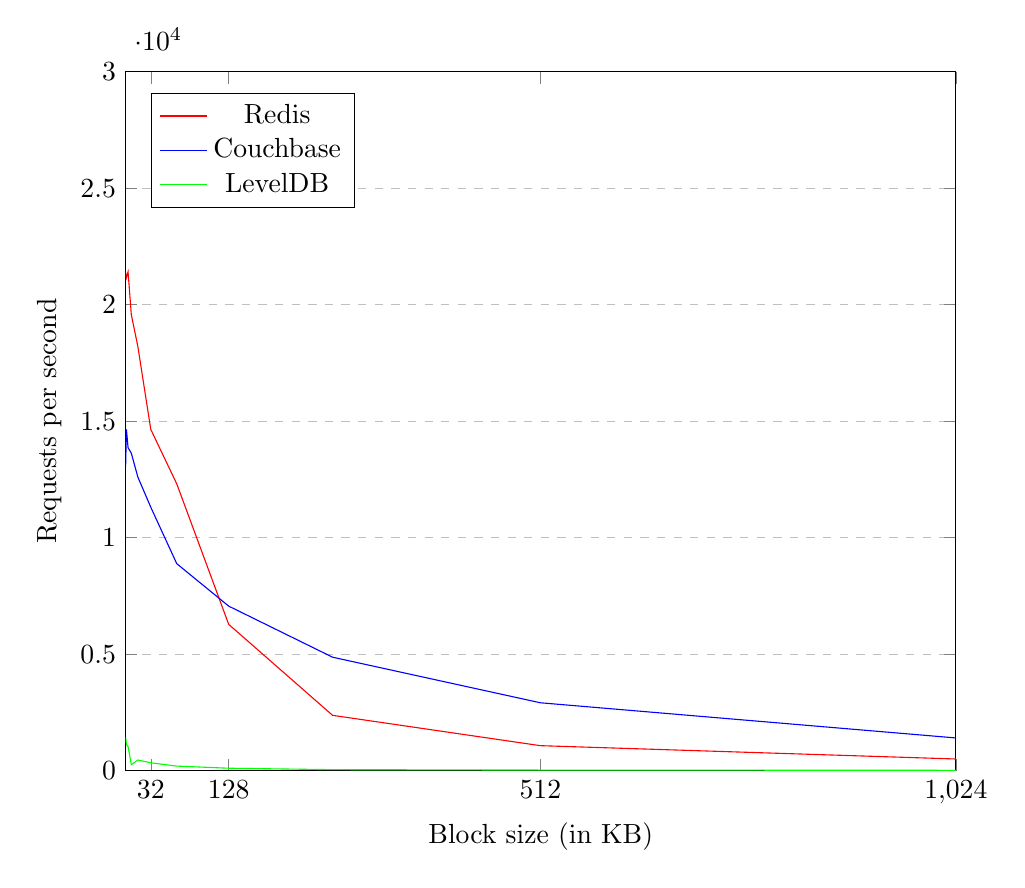
\begin{tikzpicture}\begin{axis}[
    %title={Performance},
    xlabel={Block size (in KB)},
    %log basis x={2},
    ylabel={Requests per second},
    xmin=1, xmax=1024,
    ymin=0, ymax=30000,
    xtick={32,128,512,1024},
    ytick={0,5000,10000,15000,20000,25000,30000},
    legend pos=north west,ymajorgrids=true,grid style=dashed,
    width=\linewidth]
% REDIS
\addplot[color=red, mark=none]
    coordinates {
    (1,21389)(2,21160)(4,21409)(8,19569)(16,18218)(32,14645)
    (64,12309)(128,6280)(256,2375)(512,1073)(1024,501)
    };\addlegendentry{Redis}
% COUCHBASE
\addplot[color=blue, mark=none]
    coordinates {
    (1,13071)(2,14643)(4,13859)(8,13627)(16,12607)
    (32,11306)(64,8884)(128,7062)(256,4870)(512,2914)(1024,1404)
    };\addlegendentry{Couchbase}
% LEVELDB
\addplot[color=green, mark=none]
    coordinates {
    (1,1440)(2,1127)(4,1040)(8,257)(16,458)(32,338)(64,196)
    (128,105)(256,43)(512,26)(1024,15)
    };\addlegendentry{LevelDB}
%\end{semilogxaxis}
\end{axis}\end{tikzpicture}
\caption{Requests per second against the block size on a single thread}
\end{figure}

% Time elapsed vs block size - to compare the time each DB spends performing the test
\begin{figure}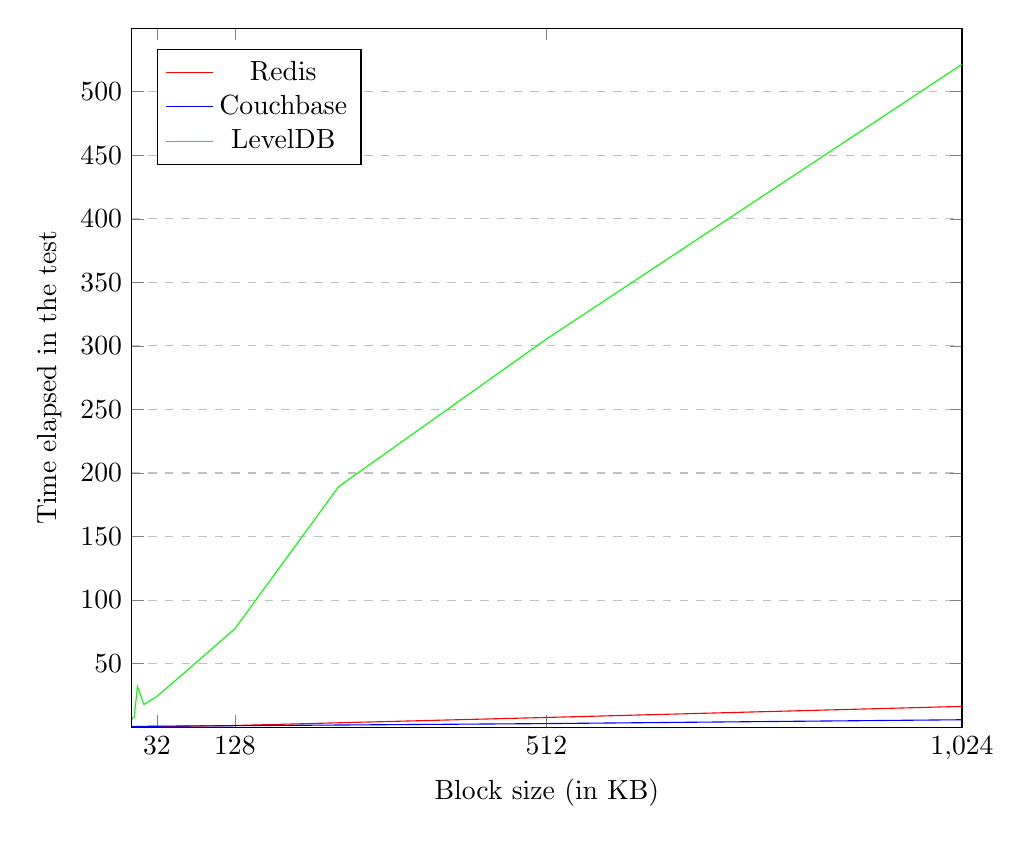
\begin{tikzpicture}\begin{axis}[
    xlabel={Block size (in KB)},
    ylabel={Time elapsed in the test},
    xmin=1, xmax=1024,
    %log basis x={2},
    ymin=0, ymax=550,
    xtick={32,128,512,1024},
    ytick={50,100,150,200,250,300,350,400,450,500},
    legend pos=north west,ymajorgrids=true,grid style=dashed,
    width=\linewidth]
% REDIS
\addplot[color=red, mark=none]
    coordinates {
    (1,0.382987)(2,0.387137)(4,0.382635)(8,0.418605)(16,0.449648)
    (32,0.559356)(64,0.665521)(128,1.30433)(256,3.44865)
    (512,7.63313)(1024,16.3394)
    };\addlegendentry{Redis}
% COUCHBASE
\addplot[color=blue, mark=none]
    coordinates {
    (1,0.626705)(2,0.559433)(4,0.591063)(8,0.601149)(16,0.649784)
    (32,0.724553)(64,0.922089)(128,1.15997)(256,1.68181)
    (512,2.81057)(1024,5.83426)
    };\addlegendentry{Couchbase}
% LEVELDB
\addplot[color=green, mark=none]
    coordinates {
    (1,5.68684)(2,7.26678)(4,7.87215)(8,31.8641)(16,17.8652)
    (32,24.1845)(64,41.777)(128,77.3897)(256,189.313)
    (512,305.396)(1024,521.602)
    };\addlegendentry{LevelDB}
\end{axis}\end{tikzpicture}
\caption{Time spent with the first stage test on a single thread}
\end{figure}

\subsubsection{Stage 2}
\subsubsection{Stage 3}
\subsubsection{Stage 1 - multithreaded}
\subsubsection{Stage 2 - multithreaded}
\subsubsection{Stage 3 - multithreaded}
\end{document}
